\documentclass[11pt,a4paper]{article}

% Paquetes esenciales
\usepackage[utf8]{inputenc}
\usepackage[spanish]{babel}
\usepackage[margin=2.5cm]{geometry}
\usepackage{graphicx}
\usepackage{fancyhdr}
\usepackage{float}
\usepackage{amsmath}
\usepackage{booktabs}
\usepackage{hyperref}
\usepackage{xcolor}
\usepackage{caption}
\usepackage{subcaption}
\usepackage{titlesec}
\usepackage{multirow}
\renewcommand{\familydefault}{\sfdefault} % sans serif
\usepackage{helvet}

% Configuración de colores
\definecolor{azuloscuro}{RGB}{0,51,102}
\definecolor{grisclaro}{RGB}{240,240,240}
\definecolor{rojochurn}{RGB}{220,53,69}
\definecolor{verdeok}{RGB}{40,167,69}

% Configuración de hipervínculos
\hypersetup{
	colorlinks=true,
	linkcolor=azuloscuro,
	filecolor=magenta,      
	urlcolor=cyan,
	citecolor=azuloscuro,
}

% Configuración de títulos de sección
\titleformat{\section}
{\normalfont\Large\bfseries\color{azuloscuro}}{\thesection}{1em}{}
\titleformat{\subsection}
{\normalfont\large\bfseries\color{azuloscuro}}{\thesubsection}{1em}{}

% Configuración del encabezado y pie de página
\pagestyle{fancy}
\fancyhf{}

\fancyhead[L]{
\includegraphics[width=4cm]{logo1.png}}
\fancyhead[R]{
\includegraphics[width=4cm]{logo2.png}}

\fancyfoot[C]{\thepage}

\setlength{\headheight}{40pt}
\renewcommand{\headrulewidth}{0.9pt}
\renewcommand{\footrulewidth}{0.9pt}

% Portada sin encabezados
\fancypagestyle{plain}{
	\fancyhf{}
	\renewcommand{\headrulewidth}{0pt}
	\fancyfoot[C]{\thepage}
}

\begin{document}
		% ==================== PORTADA ====================
	\begin{titlepage}
		\centering
		\vspace*{1cm}
		
\includegraphics[width=2.5cm]{logo1.png}
		\hfill
		
\includegraphics[width=2.5cm]{logo2.png}		
		\vspace{2cm}
		
		{\Huge\bfseries\color{azuloscuro} Reporte Ejecutivo\par}
		\vspace{0.5cm}
		{\LARGE\textbf {Análisis Predictivo en Finanzas}\par}
		{\Large\textbf{MBD00011 - Magíster en Business Analytics}\par}
		
		
		
		\vfill
		
		{\large Daniel Avello - Felipe Valdivia - Roberto Sepúlveda\par}
		\vspace{0.3cm}
		{\large \today\par}
		
	\end{titlepage}

	
	% =====================
	\section*{Resumen}
	\addcontentsline{toc}{section}{Resumen}
	
	El presente informe evalúa la predictibilidad en series financieras mediante la integración de simulaciones, modelos econométricos de series de tiempo y evidencia empírica en el contexto de la literatura de commodity currencies.

	En la Parte 1, se analizan las propiedades estadísticas de procesos estocásticos bajo distintos niveles de persistencia, evidenciando el problema de regresión espuria en presencia de no estacionariedad. Los resultados muestran que, a medida que aumenta la persistencia de las series, se incrementa la frecuencia de falsos rechazos, incluso cuando las variables son independientes, destacando la importancia de trabajar con series estacionarias.

	En la Parte 2, se examina la capacidad predictiva de los tipos de cambio sobre los precios de commodities, utilizando tanto evaluaciones in-sample como out-of-sample, junto con métricas estadísticas y económicas de desempeño. Los resultados indican que, si bien existe evidencia de predictibilidad in-sample consistente con la literatura, esta depende críticamente de la especificación del modelo y no se mantiene de forma robusta en ejercicios fuera de muestra.
	
	Asimismo, la evaluación económica basada en Mean Directional Accuracy y estrategias de trading muestra que dicha predictibilidad no se traduce en beneficios económicos significativos. Adicionalmente, se analiza la paradoja del MSPE, evidenciando que distintas métricas pueden generar conclusiones divergentes sobre el desempeño predictivo.

	En la Parte 3, se modela la dinámica del GDP mediante la metodología Box-Jenkins, confirmando la presencia de integración de orden uno y la adecuación de modelos ARIMA para capturar su comportamiento temporal. Los resultados muestran que el modelo seleccionado cumple con los supuestos de especificación y presenta residuos consistentes con ruido blanco.
	
	En conjunto, los resultados destacan la importancia de la estacionariedad, la evaluación fuera de muestra y la interpretación económica en el análisis predictivo, mostrando que la predictibilidad en finanzas es limitada, dependiente de la especificación y difícil de explotar de manera sistemática.
.
	\newpage
	% =====================
	\section{Introducción}
	
	La predicción en mercados financieros ha sido un tema central en la literatura de econometría y finanzas, particularmente en el contexto de la hipótesis de eficiencia de los mercados y la dificultad de explotar patrones sistemáticos en los datos. En este marco, la identificación de relaciones predictivas entre variables económicas y financieras requiere no solo herramientas econométricas adecuadas, sino también un tratamiento riguroso de las propiedades estadísticas de las series de tiempo.

	Uno de los principales desafíos en este tipo de análisis es la presencia de no estacionariedad, la cual puede generar inferencias engañosas a través de fenómenos como la regresión espuria. Este problema ha sido ampliamente documentado en la literatura y constituye un punto de partida fundamental para cualquier ejercicio de modelación en series financieras. Asimismo, la evaluación de modelos predictivos debe realizarse más allá del ajuste dentro de muestra, incorporando análisis fuera de muestra que permitan validar la estabilidad y relevancia de los resultados en contextos más realistas.

	En este contexto, la literatura de commodity currencies ha planteado que los tipos de cambio de economías exportadoras pueden contener información anticipada sobre los precios de commodities, dado su carácter forward-looking. Sin embargo, la evidencia empírica muestra que esta capacidad predictiva no es necesariamente robusta, dependiendo de la especificación del modelo, del horizonte de predicción y del criterio de evaluación utilizado.

	El presente informe aborda estos desafíos mediante un enfoque integral que combina simulaciones, análisis empírico y modelación de series de tiempo. 

	En la Parte 1, se analizan las implicancias de la no estacionariedad a través de simulaciones de procesos AR(1), mostrando cómo la persistencia de las series afecta la validez de la inferencia estadística. 

	En la Parte 2, se evalúa empíricamente la hipótesis de commodity currencies, analizando la capacidad predictiva de los tipos de cambio sobre precios de commodities mediante distintos enfoques de evaluación, tanto estadísticos como económicos.

 	Finalmente, en la Parte 3, se aplica la metodología Box-Jenkins para modelar la dinámica del GDP, enfatizando la importancia de la identificación de raíces unitarias y la correcta especificación de modelos ARIMA.
 
	En conjunto, este trabajo busca no solo evaluar la existencia de predictibilidad en mercados financieros, sino también destacar las limitaciones prácticas asociadas a su identificación y explotación, enfatizando la importancia de la estacionariedad, la evaluación fuera de muestra y la interpretación económica de los resultados.

	\newpage
	% =====================
	\section{Simulaciones y Regresión Espuria}
	
	\subsection{Metodología}
	
	Se simulan procesos autorregresivos de orden uno, AR(1), bajo tres escenarios que difieren en su grado de persistencia: un caso estacionario, un caso altamente persistente y un caso de caminata aleatoria. Esta clasificación permite analizar cómo las propiedades estadísticas de las series afectan la validez de la inferencia econométrica.
	
	Posteriormente, se estiman regresiones lineales entre variables generadas de manera independiente, de la forma:	
	\begin{equation}
		Y_t = c + k X_t + \varepsilon_t
	\end{equation}
	
	donde, por construcción, el parámetro k es igual a cero, lo que implica que no existe relación económica entre las variables. Este diseño permite evaluar la frecuencia de falsos rechazos de la hipótesis nula bajo distintos niveles de persistencia.
	
	\subsection{Resultados}
	De acuerdo con la evidencia reportada en las Tablas
\begin{table}[H]
	\centering
	\caption{Resultados de Regresión: AR(1) estacionario ($b = 0.6$)}
	\label{tab:res_i}
	\begin{tabular}{lrrrrrr}
		\toprule
		Regresión & $\hat{k}$ & p-val(usual) & Sig. (usual) & p-val(HAC) & Sig. (HAC) & $R^2$ \\
		\midrule
		$Y_1 \sim X_1$   & 0.0966  & 0.0030 & Sí  & 0.0356 & Sí  & 0.0088 \\
		$Y_2 \sim X_2$   & -0.0212 & 0.4925 & No  & 0.6301 & No  & 0.0005 \\
		$Y_3 \sim X_3$   & 0.0158  & 0.6445 & No  & 0.7331 & No  & 0.0002 \\
		$Y_4 \sim X_4$   & 0.0651  & 0.0403 & Sí  & 0.1148 & No  & 0.0042 \\
		$Y_5 \sim X_5$   & 0.0286  & 0.3711 & No  & 0.5178 & No  & 0.0008 \\
		$Y_6 \sim X_6$   & 0.0349  & 0.2996 & No  & 0.4614 & No  & 0.0011 \\
		$Y_7 \sim X_7$   & -0.0012 & 0.9699 & No  & 0.9808 & No  & 0.0000 \\
		$Y_8 \sim X_8$   & 0.0511  & 0.1027 & No  & 0.2204 & No  & 0.0027 \\
		$Y_9 \sim X_9$   & -0.0729 & 0.0285 & Sí  & 0.1444 & No  & 0.0048 \\
		$Y_{10} \sim X_{10}$ & -0.1091 & 0.0007 & Sí  & 0.0034 & Sí  & 0.0115 \\
		\bottomrule
	\end{tabular}
\end{table}
\begin{table}[H]
	\centering
	\caption{Resultados de Regresión: AR(1) altamente persistente ($b = 0.97$)}
	\label{tab:res_ii}
	\begin{tabular}{lrrrrrr}
		\toprule
		Regresión & $\hat{k}$ & p-val(usual) & Sig. (usual) & p-val(HAC) & Sig. (HAC) & $R^2$ \\
		\midrule
		$Y_1 \sim X_1$   & -0.0956 & 0.0188 & Sí  & 0.4146 & No  & 0.0055 \\
		$Y_2 \sim X_2$   & -0.0028 & 0.9365 & No  & 0.9810 & No  & 0.0000 \\
		$Y_3 \sim X_3$   & -0.0654 & 0.1237 & No  & 0.6442 & No  & 0.0024 \\
		$Y_4 \sim X_4$   & 0.1037  & 0.0003 & Sí  & 0.1858 & No  & 0.0130 \\
		$Y_5 \sim X_5$   & -0.0526 & 0.1726 & No  & 0.6325 & No  & 0.0019 \\
		$Y_6 \sim X_6$   & 0.2289  & 0.0000 & Sí  & 0.2220 & No  & 0.0185 \\
		$Y_7 \sim X_7$   & 0.0294  & 0.3291 & No  & 0.6882 & No  & 0.0010 \\
		$Y_8 \sim X_8$   & -0.0091 & 0.7592 & No  & 0.9179 & No  & 0.0001 \\
		$Y_9 \sim X_9$   & -0.2760 & 0.0000 & Sí  & 0.0003 & Sí  & 0.0846 \\
		$Y_{10} \sim X_{10}$ & -0.1381 & 0.0000 & Sí  & 0.0607 & Sí  & 0.0291 \\
		\bottomrule
	\end{tabular}
\end{table}
\begin{table}[H]
	\centering
	\caption{Resultados de Regresión: Caminata Aleatoria (Random Walk)}
	\label{tab:res_iii}
	\begin{tabular}{lrrrrrr}
		\toprule
		Regresión & $\hat{k}$ & p-val(usual) & Sig.(usual) & p-val(HAC) & Sig. (HAC) & $R^2$ \\
		\midrule
		$Y_1 \sim X_1$   & -0.5218 & 0.0000 & Sí  & 0.0001 & Sí  & 0.1849 \\
		$Y_2 \sim X_2$   & -0.1082 & 0.0000 & Sí  & 0.2221 & No  & 0.0204 \\
		$Y_3 \sim X_3$   & 1.0138  & 0.0000 & Sí  & 0.0000 & Sí  & 0.5859 \\
		$Y_4 \sim X_4$   & 0.0713  & 0.0351 & Sí  & 0.4228 & No  & 0.0044 \\
		$Y_5 \sim X_5$   & 0.4358  & 0.0000 & Sí  & 0.0000 & Sí  & 0.2731 \\
		$Y_6 \sim X_6$   & 0.5454  & 0.0000 & Sí  & 0.0012 & Sí  & 0.2204 \\
		$Y_7 \sim X_7$   & 0.3302  & 0.0000 & Sí  & 0.0000 & Sí  & 0.4135 \\
		$Y_8 \sim X_8$   & 0.2598  & 0.0000 & Sí  & 0.0009 & Sí  & 0.1209 \\
		$Y_9 \sim X_9$   & 0.2076  & 0.0000 & Sí  & 0.0118 & Sí  & 0.0582 \\
		$Y_{10} \sim X_{10}$ & -1.0607 & 0.0000 & Sí  & 0.0000 & Sí  & 0.7014 \\
		\bottomrule
	\end{tabular}
\end{table}
\begin{figure}[H]
	\centering		
	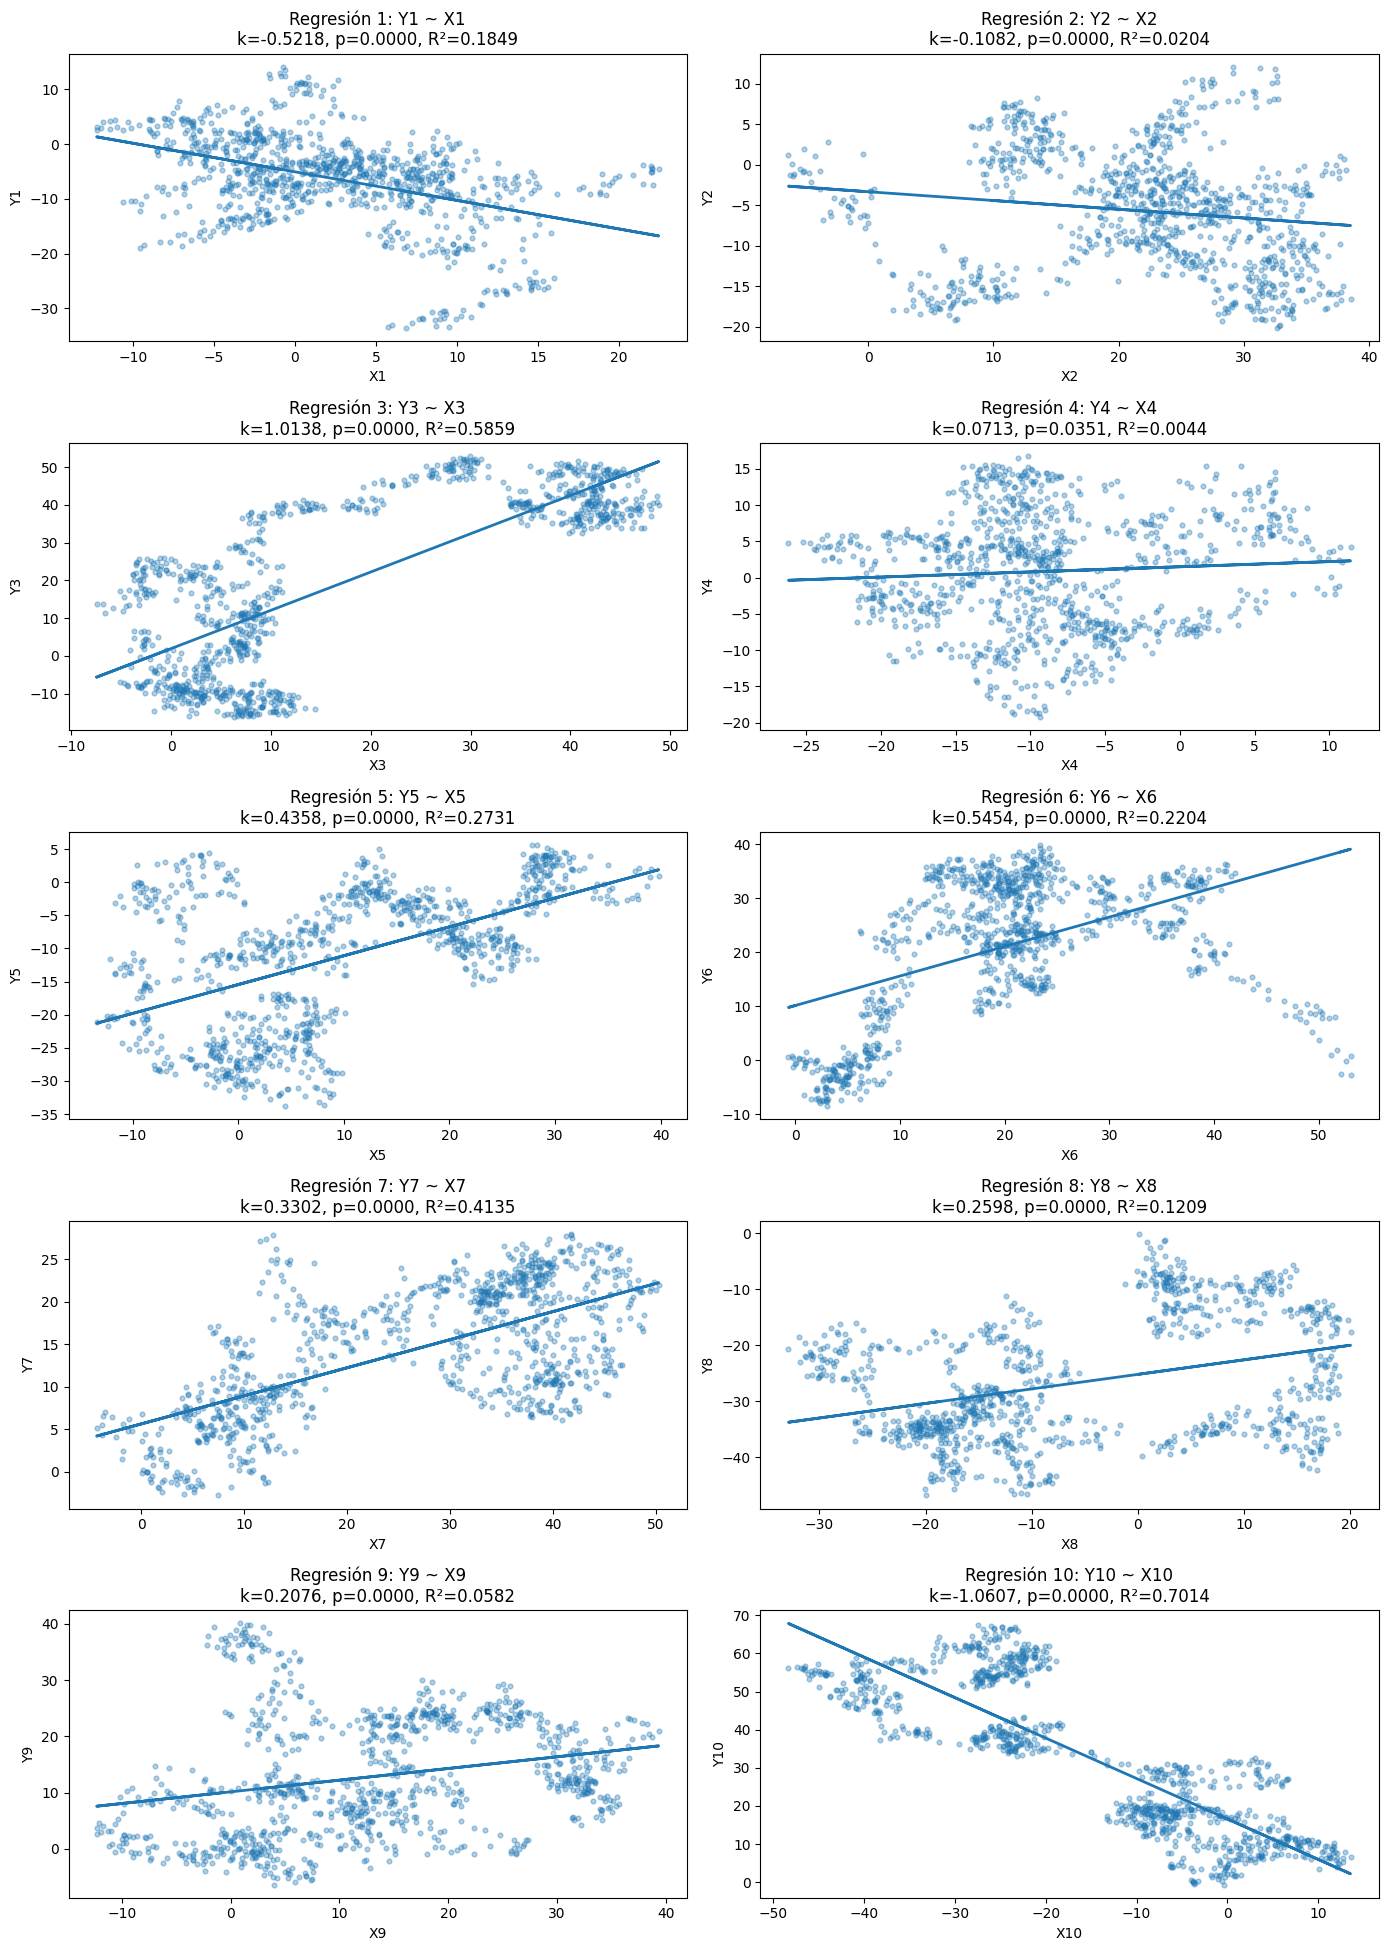
\includegraphics[width=0.9\textwidth]{Pregunta_iii_Random_Walk.png}		
	\caption{Regresiones Random Walk, b=1}
	\label{fig:diagnostico_residuos}		
\end{figure}

\begin{table}[H]
	\centering
	\caption{Resumen Consolidado de Resultados de Simulación}
	\label{tab:resumen_final}
	\begin{tabular}{lllrrrr}
		\toprule
		Escenario & Valor de $b$ & Nivel & \%(usual) & \%(HAC) & $R^2$ prom. & $R^2$ máx \\
		\midrule
		i) AR(1) estacionario & 0.6 & 10\% & 40.0 & 20.0 & 0.0035 & 0.0115 \\
		ii) AR(1) altamente persistente & 0.97 & 10\% & 50.0 & 20.0 & 0.0156 & 0.0846 \\
		iii) Random Walk & 1.0 & 5\% & 100.0 & 80.0 & 0.2583 & 0.7014 \\
		\bottomrule
	\end{tabular}
\end{table}
	
	se observa que la proporción de rechazos de la hipótesis nula $H_0: k = 0$ aumenta sistemáticamente con el grado de persistencia del proceso generador de datos.
	En particular, se identifican tres patrones claramente diferenciados. En el caso estacionario, la proporción de rechazos presenta variabilidad, la cual puede atribuirse principalmente al reducido número de simulaciones realizadas. En el caso altamente persistente, la frecuencia de falsos positivos aumenta de manera significativa, reflejando el impacto de la autocorrelación sobre la inferencia estadística. Finalmente, en el caso de caminata aleatoria, la proporción de rechazos es prácticamente total, a pesar de la independencia entre las variables, lo que constituye evidencia directa de regresión espuria. frecuencia de falsos rechazos de la hipótesis nula bajo distintos niveles de persistencia.
	
	
	\subsection{Interpretación}	
	Los resultados obtenidos constituyen evidencia clara del fenómeno de regresión espuria, el cual surge cuando se estiman relaciones entre series no estacionarias. En estos casos, los estadísticos de prueba, como el estadístico t asociado al parámetro k, no siguen sus distribuciones asintóticas estándar, lo que invalida la inferencia tradicional.
	
	A medida que aumenta la persistencia de los procesos, la autocorrelación introduce dependencia temporal que distorsiona la estimación de la varianza de los errores. Como consecuencia, los errores estándar tienden a subestimarse, lo que incrementa artificialmente la significancia estadística de los coeficientes estimados. Este efecto se vuelve especialmente pronunciado en el caso de caminatas aleatorias, donde la presencia de raíz unitaria genera trayectorias altamente persistentes que inducen correlaciones espurias entre variables independientes.
	
	Si bien el uso de errores estándar robustos, como los estimadores HAC, permite corregir parcialmente problemas asociados a heterocedasticidad y autocorrelación, estos no resuelven el problema fundamental de la no estacionariedad. Por lo tanto, incluso con ajustes robustos, la inferencia puede seguir siendo inválida cuando las series presentan raíces unitarias.

	
	\subsection{Conclusión}
	
	La evidencia obtenida confirma que la estacionariedad constituye una condición necesaria para realizar inferencia econométrica válida en series de tiempo. En particular, se observa que la presencia de alta persistencia y, especialmente, de raíces unitarias conduce a un aumento significativo en la frecuencia de falsos rechazos de la hipótesis nula, aun cuando las variables sean independientes.
	
	Estos resultados ilustran empíricamente el fenómeno de regresión espuria, en el cual se obtienen relaciones aparentemente significativas que carecen de fundamento económico. En consecuencia, ignorar la estacionariedad de las series puede llevar a conclusiones erróneas y a una interpretación equivocada de los resultados econométricos.
	
	Por lo tanto, el análisis de raíces unitarias y la transformación adecuada de las series deben considerarse pasos indispensables en cualquier ejercicio de modelación y predicción en datos de series de tiempo.

	\newpage
	% =====================
	\section{Commodity Currencies}
	
	\subsection{Motivación}
	
	La literatura de commodity currencies plantea que los tipos de cambio de economías exportadoras de materias primas contienen información anticipada sobre los precios futuros de dichos commodities. Esta relación se sustenta en el hecho de que el tipo de cambio es una variable forward-looking, que incorpora expectativas sobre fundamentos económicos futuros, incluyendo términos de intercambio, demanda global y condiciones del mercado de commodities.
	
	En este contexto, variaciones en los precios esperados de commodities pueden reflejarse tempranamente en el tipo de cambio, generando una posible relación predictiva desde el tipo de cambio hacia los precios de los commodities. Esta hipótesis ha sido documentada en la literatura empírica, donde se encuentra evidencia de predictibilidad en ciertos horizontes y para economías específicas.
	
	No obstante, la evidencia no es concluyente, ya que la capacidad predictiva depende de la especificación del modelo, del horizonte de predicción y del criterio de evaluación utilizado, especialmente cuando se consideran ejercicios fuera de muestra.

	
	\subsection{Estacionariedad}
	De acuerdo con los resultados reportados en la Tabla Raíz Unitaria ADF, las series en niveles presentan evidencia de no estacionariedad, consistente con la presencia de raíz unitaria. En contraste, las primeras diferencias logarítmicas, interpretadas como retornos, muestran un comportamiento estacionario.
\begin{table}[H]
	\centering
	\caption{Resultados del Test de Raíz Unitaria ADF}
	\label{tab:adf}
	
	\small
	
	\begin{tabular}{llrrr}
		\toprule
		Serie & Transformación &ADF Stat &p-value &Rechaza RU 5\% \\
		\midrule		
		chile & Nivel &-1.4589 & 0.5537 & False \\		
		chile & Logaritmo &-1.4982 & 0.5344 & False \\		
		chile & Retorno log &-15.4096 & 0.0000 & True \\		
		australia & Nivel &-1.5188 & 0.5242 & False \\		
		australia & Logaritmo &-1.5412 & 0.5131 & False \\		
		australia & Retorno log &-15.0744 & 0.0000 & True \\		
		copper & Nivel &-2.0839 & 0.2510 & False \\		
		copper & Logaritmo &-1.8214 & 0.3699 & False \\		
		copper & Retorno log &-8.6658 & 0.0000 & True \\		
		aluminum & Nivel &-2.2837 & 0.1773 & False \\		
		\bottomrule
	\end{tabular}

\end{table}
\begin{figure}[H]
	\centering		
	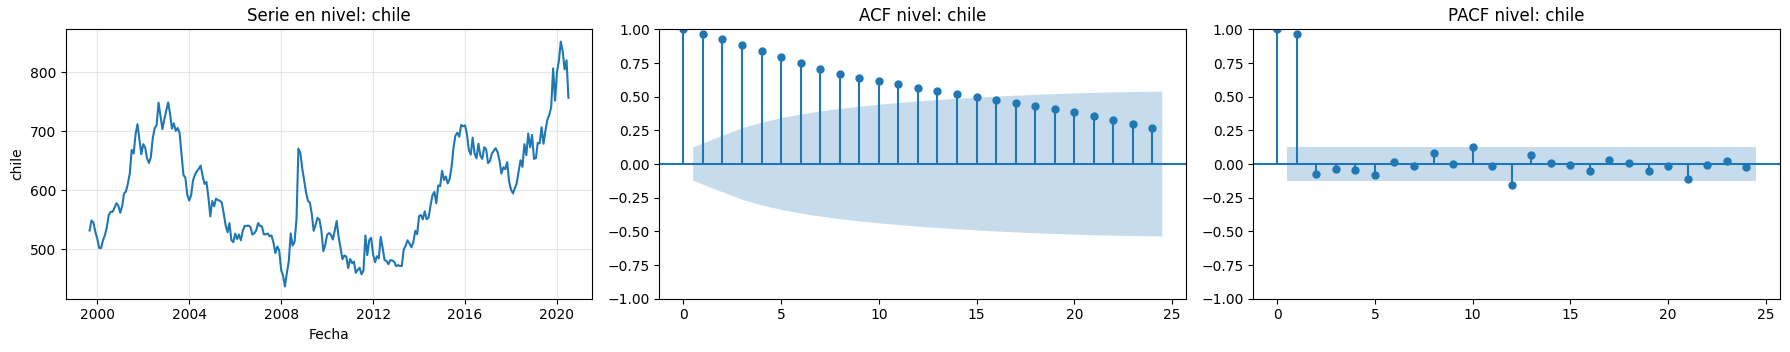
\includegraphics[width=0.9\textwidth]{grafico_1_Nivel_ACF_PACF_chile.png}		
	\caption{Nivel ACF y PACF chile}
	\label{fig:diagnostico_residuos}		
\end{figure}
\begin{figure}[H]
	\centering		
	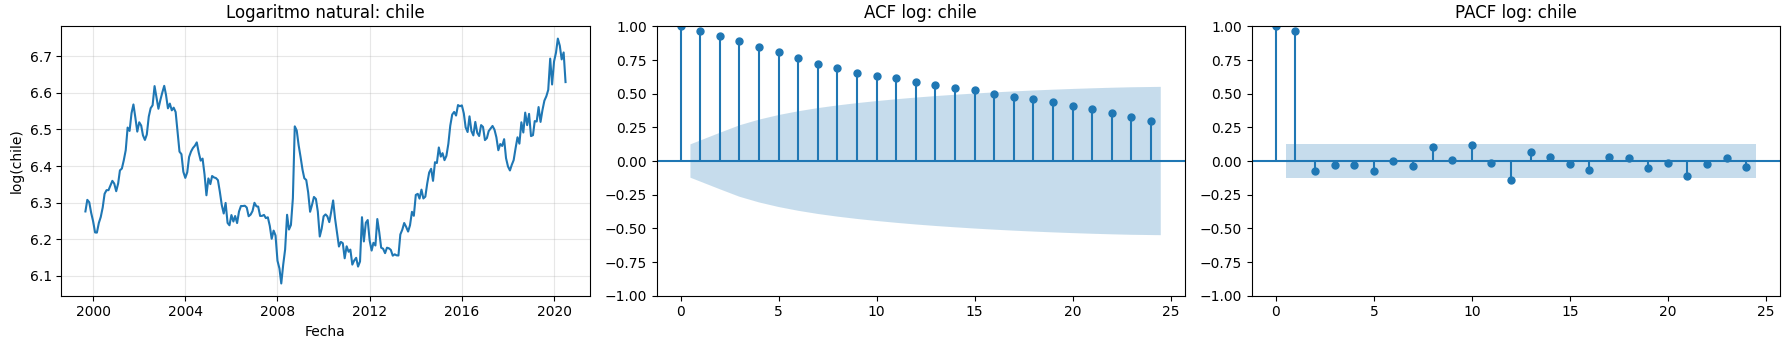
\includegraphics[width=0.9\textwidth]{grafico_2_Log_ACF_PACF_chile.png}		
	\caption{Logaritmo natural, ACF y PACF para: Chile}
	\label{fig:diagnostico_residuos}		
\end{figure}
\begin{figure}[H]
	\centering		
	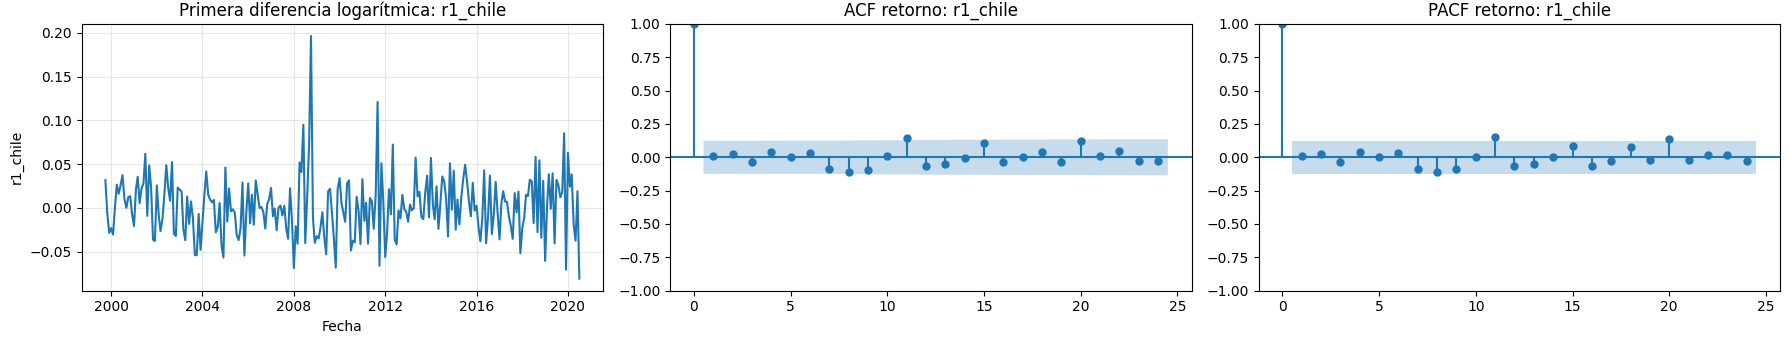
\includegraphics[width=0.9\textwidth]{grafico_3_Retornos_ACF_PACF_r1_chile.png}		
	\caption{Retorno Logarítmico 1 mes, ACF y PACF para : R1 Chile}
	\label{fig:diagnostico_residuos}		
\end{figure}
	Este resultado es coherente con la evidencia empírica en finanzas, donde los precios de activos suelen modelarse como procesos integrados de orden uno, $I(1)$, mientras que sus retornos son aproximadamente estacionarios. Desde un punto de vista econométrico, trabajar con variables no estacionarias puede conducir a problemas de regresión espuria, afectando la validez de la inferencia.

	Por esta razón, el análisis predictivo se realiza sobre las diferencias logarítmicas de las series:
	
	\begin{equation}
		\Delta \log(P_t)
	\end{equation}
	lo que permite asegurar que las propiedades estadísticas de las variables sean compatibles con los supuestos de los modelos utilizados.
	\subsection{Resultados In-Sample}
	De acuerdo con los resultados reportados en las Tablas:
\begin{table}[H]
	\centering
	\caption{Resultados Predictivos In-Sample (Chen, Rogoff y Rossi)}
	\label{tab:res_e}
	
	\resizebox{\textwidth}{!}{
		\begin{tabular}{llrrrrrrrrr}
			\toprule
			Commodity & TC & $\rho$ AR & p-val $\rho$ & Sig. $\rho$ &
			$\beta_{TC}$ & p-val $\beta$ & Sig. $\beta$ &
			$R^2_{AR}$ & $R^2_{CRR}$ & $\Delta R^2$ \\
			\midrule			
			copper   & chile      & 0.1166 & 0.1106 & False & -0.2067 & 0.1962 & False & 0.0269 & 0.0335 & 0.0066 \\
			copper   & australia  & 0.1190 & 0.1195 & False & -0.1643 & 0.2938 & False & 0.0269 & 0.0313 & 0.0044 \\			
			aluminum & chile      & -0.0284 & 0.6750 & False & -0.2883 & 0.0136 & True & 0.0011 & 0.0256 & 0.0245 \\
			aluminum & australia  & -0.0650 & 0.3686 & False & -0.3199 & 0.0061 & True & 0.0011 & 0.0313 & 0.0302 \\			
			lmex     & chile      & 0.0835 & 0.2641 & False & -0.2114 & 0.1157 & False & 0.0214 & 0.0312 & 0.0098 \\
			lmex     & australia  & 0.0716 & 0.3715 & False & -0.2041 & 0.1300 & False & 0.0214 & 0.0305 & 0.0091 \\			
			\bottomrule
		\end{tabular}
	}
	
\end{table} 
\begin{table}[H]
	\centering
	\caption{Resultados Predictivos In-Sample con Errores HAC (Modelo F)}
	\label{tab:res_f}
	
	\resizebox{\textwidth}{!}{
		\begin{tabular}{llrrrrrrrrr}
			\toprule
			Commodity & TC & $\rho$ AR & p-val $\rho$ & Sig. $\rho$ &
			$\beta_{TC}$ & p-val $\beta$ & Sig. $\beta$ &
			$R^2_{AR}$ & $R^2_{HAC}$ & $\Delta R^2$ \\
			\midrule			
			copper   & chile      & 0.1166 & 0.2201 & False & -0.2067 & 0.2177 & False & 0.0269 & 0.0335 & 0.0066 \\
			copper   & australia  & 0.1190 & 0.2351 & False & -0.1643 & 0.3715 & False & 0.0269 & 0.0313 & 0.0044 \\			
			aluminum & chile      & -0.0284 & 0.7568 & False & -0.2883 & 0.0342 & True & 0.0011 & 0.0256 & 0.0245 \\
			aluminum & australia  & -0.0650 & 0.5406 & False & -0.3199 & 0.0414 & True & 0.0011 & 0.0313 & 0.0302 \\			
			lmex     & chile      & 0.0835 & 0.3992 & False & -0.2114 & 0.1418 & False & 0.0214 & 0.0312 & 0.0098 \\
			lmex     & australia  & 0.0716 & 0.5015 & False & -0.2041 & 0.2009 & False & 0.0214 & 0.0305 & 0.0091 \\			
			\bottomrule
		\end{tabular}
	}
	
\end{table}
		se observa evidencia de predictibilidad en varios casos, particularmente cuando se utiliza el tipo de cambio chileno como variable explicativa. En estas especificaciones, algunos coeficientes resultan estadísticamente significativos, lo que sugiere la existencia de relaciones predictivas dentro de la muestra.

	\subsection{Interpretación}
		Si bien estos resultados son consistentes con la literatura de commodity currencies, su interpretación debe realizarse con cautela. La significancia estadística in-sample puede estar influenciada por factores como la persistencia de las series, la correlación serial y el potencial sobreajuste de los modelos a los datos observados.
		
		En particular, un buen desempeño dentro de muestra no garantiza capacidad predictiva fuera de muestra, ya que los modelos pueden capturar patrones específicos del período analizado que no se mantienen en el tiempo. Por lo tanto, estos resultados deben considerarse como evidencia preliminar de predictibilidad, cuya validez debe ser evaluada mediante análisis out-of-sample.
\newpage
	
	\subsection{Resultados Out-of-Sample}
	
	De acuerdo con los resultados reportados en las Tablas:
	\begin{table}[H]
		\centering
		\caption{Resultados Fuera de Muestra (División 30\%-70\%)}
		\label{tab:oos_30}
		
		\resizebox{\textwidth}{!}{
			\begin{tabular}{llllrrrrrr}
				\toprule
				Commodity & TC & Ventana & Modelo &
				ECM & $R^2_{OOS}$ &
				DM Stat &
				p-value DM &
				Sig. 5\% &
				Mejor que AR(1) \\
				\midrule				
				copper & chile & recursive & PH dos rezagos &
				0.0064 & -0.0077 & 0.2792 & 0.7801 & False & False \\				
				copper & chile & recursive & AR(1) &
				0.0064 & 0.0000 & NaN & NaN & False & False \\				
				copper & chile & recursive & Promedio histórico &
				0.0064 & -0.0087 & 0.1615 & 0.8717 & False & False \\				
				copper & chile & recursive & Zero forecast &
				0.0063 & 0.0066 & -0.1369 & 0.8911 & False & True \\				
				copper & chile & rolling & PH dos rezagos &
				0.0065 & -0.0126 & 0.4521 & 0.6512 & False & False \\				
				copper & chile & rolling & AR(1) &
				0.0065 & 0.0000 & NaN & NaN & False & False \\				
				copper & chile & rolling & Promedio histórico &
				0.0065 & -0.0053 & 0.0785 & 0.9374 & False & False \\				
				copper & chile & rolling & Zero forecast &
				0.0063 & 0.0184 & -0.3084 & 0.7578 & False & True \\				
				copper & australia & recursive & PH dos rezagos &
				0.0066 & -0.0417 & 1.1512 & 0.2496 & False & False \\				
				copper & australia & recursive & AR(1) &
				0.0064 & 0.0000 & NaN & NaN & False & False \\				
				\bottomrule
			\end{tabular}
		}
		
	\end{table}
	\begin{table}[H]
		\centering
		\caption{Resultados Fuera de Muestra (División 50\%-50\%)}
		\label{tab:oos_50}
		
		\resizebox{\textwidth}{!}{
			\begin{tabular}{llllrrrrrr}
				\toprule
				Commodity & TC & Ventana & Modelo &
				ECM & $R^2_{OOS}$ &
				DM Stat &
				p-value DM &
				Sig. 5\% &
				Mejor que AR(1) \\
				\midrule				
				copper & chile & recursive & PH dos rezagos &0.0043 & -0.0238 & 0.5464 & 0.5848 &False & False \\				
				copper & chile & recursive & AR(1) &0.0042 & 0.0000 & NaN & NaN & False & False \\				
				copper & chile & recursive & Promedio histórico &0.0037 & 0.1020 & -1.9898 & 0.0466 & True & True \\				
				copper & chile & recursive & Zero forecast &0.0036 & 0.1287 & -2.2827 & 0.0225 & True & True \\				
				copper & chile & rolling & PH dos rezagos &0.0044 & -0.0246 & 0.5687 & 0.5696 & False & False \\				
				copper & chile & rolling & AR(1) &0.0043 & 0.0000 & NaN & NaN & False & False \\				
				copper & chile & rolling & Promedio histórico &	0.0038 & 0.1098 & -2.0987 & 0.0358 & True & True \\				
				copper & chile & rolling & Zero forecast &0.0036 & 0.1498 & -2.5515 & 0.0107 & True & True \\				
				copper & australia & recursive & PH dos rezagos &0.0042 & -0.0074 & 0.4548 & 0.6492 & False & False \\				
				copper & australia & recursive & AR(1) &0.0042 & 0.0000 & NaN & NaN & False & False \\				
				\bottomrule
			\end{tabular}
		}
		
	\end{table}
	la evidencia de predictibilidad fuera de muestra es, en general, mixta. En particular, los modelos que incorporan el tipo de cambio chileno como variable explicativa no logran superar de manera consistente al benchmark AR(1), independientemente de la partición de la muestra utilizada.
	
	Si bien en algunos casos específicos se observan mejoras en términos de error de predicción, estas no son sistemáticas ni robustas a lo largo de distintos horizontes o especificaciones. Esto sugiere que la capacidad predictiva identificada en los ejercicios in-sample no se mantiene de forma estable cuando se evalúa en datos no utilizados para la estimación.
	
	\subsection{Interpretación}
	Los resultados out-of-sample constituyen una evaluación más exigente y realista de la capacidad predictiva de los modelos. A diferencia del análisis in-sample, donde los parámetros se estiman utilizando toda la información disponible, la evaluación fuera de muestra permite identificar si las relaciones estimadas son estables y generalizables en el tiempo.
	
	En este contexto, la ausencia de una mejora consistente respecto a modelos benchmark simples, como el AR(1), indica que la predictibilidad observada dentro de muestra puede estar asociada a sobreajuste o a características específicas del período analizado. Por lo tanto, no es posible afirmar que exista evidencia robusta de predictibilidad en términos econométricos.
\newpage	
	\subsection{Evaluación Económica (MDA y Trading)}	
	De acuerdo con los resultados presentados en las Tablas: 
	\begin{table}[H]
		\centering
		\caption{Resultados de Mean Directional Accuracy (MDA)}
		\label{tab:mda}
		
		\resizebox{\textwidth}{!}{
			\begin{tabular}{llllrrrr}
				\toprule
				Commodity & TC & Ventana & Modelo &
				MDA &
				Stat vs 50\% &
				p-value unilateral &
				Supera pure luck \\
				\midrule				
				copper & chile & recursive&PH dos rezagos &0.4597 & -0.8265 & 0.7957 & False\\				
				copper & chile & recursive&AR(1) &0.4194 &-1.7717 & 0.9618 & False\\				
				copper & chile&recursive&Promediohistórico&0.5081&0.1963&0.4222&False\\				
				copper & chile & recursive& Zero forecast &0.0000 & NaN & NaN & False\\				
				copper & chile & rolling & PH dos rezagos &0.4677 & -0.6968 & 0.7570 & False\\				
				copper & chile & rolling & AR(1) &0.4597 & -0.9107 & 0.8188 & False \\				
				copper & chile & rolling & Promedio histórico &0.5000 & 0.0000 & 0.5000 & False \\				
				copper & chile & rolling & Zero forecast &0.0000 & NaN & NaN & False \\				
				copper & australia & recursive & PH dos rezagos &0.4194 & -1.7342 & 0.9586 & False \\				
				copper & australia & recursive & AR(1) &0.4194 & -1.7717 & 0.9618 & False \\				
				\bottomrule
			\end{tabular}
		}
		
	\end{table}
	\begin{table}[H]
		\centering
		\caption{Rentabilidad de Estrategia de Trading (Anatolyev y Gerko)}
		\label{tab:trading}
		
		\resizebox{\textwidth}{!}{
			\begin{tabular}{llllrrrrr}
				\toprule
				Commodity & TC & Ventana & Modelo &
				Retorno medio &
				Retorno anualizado &
				$t$-stat HAC &
				p-value HAC &
				Rentabilidad significativa \\
				\midrule				
				copper & chile & recursive & PH dos rezagos &
				0.0007 & 0.0088 & 0.1598 & 0.8731 & False \\				
				copper & chile & recursive & AR(1) &
				-0.0052 & -0.0622 & -1.1098 & 0.2671 & False \\				
				copper & chile & recursive & Promedio histórico &
				-0.0015 & -0.0183 & -0.3169 & 0.7513 & False \\				
				copper & chile & recursive & Zero forecast &
				0.0000 & 0.0000 & NaN & NaN & False \\				
				copper & chile & rolling & PH dos rezagos &
				0.0011 & 0.0133 & 0.2356 & 0.8137 & False \\				
				copper & chile & rolling & AR(1) &
				-0.0042 & -0.0505 & -0.8107 & 0.4175 & False \\				
				copper & chile & rolling & Promedio histórico &
				-0.0074 & -0.0891 & -1.4903 & 0.1361 & False \\				
				copper & chile & rolling & Zero forecast &
				0.0000 & 0.0000 & NaN & NaN & False \\				
				copper & australia & recursive & PH dos rezagos &
				-0.0042 & -0.0505 & -0.8743 & 0.3820 & False \\				
				copper & australia & recursive & AR(1) &
				-0.0052 & -0.0622 & -1.1098 & 0.2671 & False \\				
				\bottomrule
			\end{tabular}
		}
		
	\end{table}
	la evidencia de predictibilidad en términos económicos es limitada. En particular, la métrica de Mean Directional Accuracy (MDA) muestra que la proporción de predicciones correctas de la dirección del retorno no supera de manera consistente el umbral del $50\%$, el cual corresponde a un desempeño equivalente a una predicción aleatoria.
	
	Asimismo, las estrategias de trading construidas a partir de los modelos predictivos no generan retornos significativamente superiores a los benchmarks considerados. En varios casos, el desempeño económico se ve afectado por la baja capacidad de anticipar correctamente la dirección de los retornos, así como por la posible presencia de costos de transacción.
	
	\subsection{Interpretación}
	Estos resultados refuerzan la idea de que la predictibilidad estadística no necesariamente se traduce en beneficios económicos. Aunque algunos modelos pueden mostrar mejoras marginales en métricas de error de predicción, estas no son suficientes para generar estrategias de inversión rentables de manera sistemática.
	
	En este sentido, la evaluación económica constituye un criterio más exigente que la evaluación puramente estadística, ya que requiere no solo precisión en la predicción, sino también capacidad de generar retornos ajustados por riesgo superiores a los benchmarks. La ausencia de evidencia robusta en términos de MDA y trading sugiere que la predictibilidad observada es débil desde una perspectiva práctica.
\newpage	
	\subsection{Bonus 1:Evaluación de Portafolio}
	Con el objetivo de evaluar la relevancia económica de la predictibilidad, se construyen estrategias de portafolio basadas en las predicciones generadas por los modelos. En particular, se utilizan los retornos esperados estimados para determinar posiciones en el activo, ajustando la exposición en función de la señal predictiva.
	
	De acuerdo con los resultados presentados en la yabla, el desempeño de las estrategias es, en general, limitado. Si bien en algunos casos se observan mejoras marginales en métricas de desempeño, estas no son consistentes ni robustas una vez que se consideran factores como la volatilidad de los retornos y los costos de transacción.
\begin{table}[H]
	\centering
	\caption{Bonus 1: Estrategia de Portafolio tipo Neely et al. (2014)}
	\label{tab:bonus1_portafolio}	
	\scriptsize
		\resizebox{\textwidth}{!}{
		\begin{tabular}{llllrrrrrrrrrr}
			\toprule
			Commodity & TC & Ventana & Modelo &
			$\gamma$ &
			$R_f$ &
			Costo &
			Ret. anual &
			Vol. anual &
			Sharpe &
			CER &
			Exceso medio &
			$t$-stat HAC &
			p-value HAC \\
			\midrule			
			copper & chile & recursive & PH dos rezagos &3 & 0.0300 & 10 &
			0.0228 & 0.2171 & -0.0313 & -0.0479 &-0.0006 & -0.1102 & 0.9123 \\			
			copper & chile & recursive & PH dos rezagos &5 & 0.0300 & 10 &
			0.0094 & 0.1820 & -0.1108 & -0.0734 &-0.0017 & -0.3782 & 0.7053 \\			
			copper & chile & recursive & AR(1) &3 & 0.0300 & 10 &
			-0.0628 & 0.1831 & -0.5043 & -0.1131 &-0.0077 & -1.7514 & 0.0799 \\			
			copper & chile & recursive & AR(1) &5 & 0.0300 & 10 &
			-0.0531 & 0.1371 & -0.6036 & -0.1001 &-0.0069 & -2.0747 & 0.0380 \\			
			copper & chile & recursive & Promedio histórico &3 & 0.0300 & 10 &
			-0.0125 & 0.1481 & -0.2846 & -0.0454 &-0.0035 & -1.0038 & 0.3155 \\			
			copper & chile & recursive & Promedio histórico &5 & 0.0300 & 10 &
			0.0025 & 0.0899 & -0.3013 & -0.0177 &-0.0023 & -1.0458 & 0.2956 \\			
			copper & chile & recursive & Zero forecast &3 & 0.0300 & 10 &
			0.0296 & 0.0000 & NaN & 0.0296 &0.0000 & NaN & NaN \\			
			copper & chile & recursive & Zero forecast &5 & 0.0300 & 10 &
			0.0296 & 0.0000 & NaN & 0.0296 &0.0000 & NaN & NaN \\			
			copper & chile & rolling & PH dos rezagos &3 & 0.0300 & 10 &
			0.0157 & 0.2107 & -0.0658 & -0.0509 &-0.0012 & -0.2166 & 0.8285 \\			
			copper & chile & rolling & PH dos rezagos &5 & 0.0300 & 10 &
			-0.0028 & 0.1679 & -0.1931 & -0.0733 &-0.0027 & -0.6282 & 0.5299 \\			
			\bottomrule
		\end{tabular}
	}
	
\end{table}
	\subsection{Interpretación}
	La ausencia de mejoras significativas en la performance del portafolio sugiere que la información contenida en los modelos predictivos no es suficiente para generar ventajas económicas sostenibles. En particular, aun cuando los modelos pueden capturar ciertas señales predictivas, estas no logran traducirse en una asignación óptima de activos que mejore de manera consistente el retorno ajustado por riesgo.
	
	Además, la incorporación de costos de transacción reduce aún más la rentabilidad de las estrategias, lo que refleja una limitación importante en la aplicabilidad práctica de los modelos. Este resultado es consistente con la literatura en finanzas empíricas, donde se documenta que la predictibilidad estadística suele ser difícil de explotar en contextos reales de inversión.
	
	\subsection{Bonus 2: Paradoja del MSPE}
	
	Con el objetivo de profundizar en la evaluación del desempeño predictivo, se analiza la denominada paradoja del MSPE, la cual surge cuando distintas métricas de evaluación entregan conclusiones aparentemente contradictorias sobre la calidad de los modelos.
	
	De acuerdo con los resultados reportados en la tabla, se observa que algunos modelos presentan un mayor error cuadrático medio de predicción (Mean Squared Prediction Error, MSPE) en comparación con modelos benchmark, pero al mismo tiempo exhiben una mayor correlación con la variable objetivo. Esta aparente contradicción refleja que diferentes métricas capturan dimensiones distintas del desempeño predictivo.
	\begin{table}[H]
		\centering
		\caption{Bonus 2: Paradoja del ECM y Test de Correlaciones}
		\label{tab:bonus2_paradoja}
		
		\scriptsize
		
		\resizebox{\textwidth}{!}{
			\begin{tabular}{lllllrrrrrrrrrr}
				\toprule
				Commodity & TC & Ventana & Modelo & Benchmark &
				ECM Modelo & ECM AR(1) &
				Peor ECM &
				Corr. Modelo &
				Corr. AR(1) &
				Mayor Corr. &
				Paradoja &
				$\Delta$ Corr. &
				p-value Boot. &
				Sig. 5\% \\
				\midrule				
				copper & chile & recursive & PH dos rezagos & AR(1) &
				0.0043 & 0.0042 & True & -0.0798 & -0.1475 & True & True & 0.0677 & 0.2953 & False \\				
				copper & chile & recursive & Promedio histórico & AR(1) &
				0.0037 & 0.0042 & False & -0.0826 & -0.1475 & True & False & 0.0649 & 0.3554 & False \\				
				copper & chile & recursive & Zero forecast & AR(1) &
				0.0036 & 0.0042 & False & NaN & -0.1475 & False & False & NaN & NaN & False \\				
				copper & chile & rolling & PH dos rezagos & AR(1) &
				0.0044 & 0.0043 & True & -0.1127 & -0.1696 & True & True & 0.0569 & 0.3724 & False \\				
				copper & chile & rolling & Promedio histórico & AR(1) &
				0.0038 & 0.0043 & False & -0.1132 & -0.1696 & True & False & 0.0564 & 0.3233 & False \\				
				copper & chile & rolling & Zero forecast & AR(1) &
				0.0036 & 0.0043 & False & NaN & -0.1696 & False & False & NaN & NaN & False \\				
				copper & australia & recursive & PH dos rezagos & AR(1) &
				0.0042 & 0.0042 & True & -0.1194 & -0.1475 & True & True & 0.0281 & 0.3834 & False \\				
				copper & australia & recursive & Promedio histórico & AR(1) &
				0.0037 & 0.0042 & False & -0.0826 & -0.1475 & True & False & 0.0649 & 0.3554 & False \\				
				copper & australia & recursive & Zero forecast & AR(1) &
				0.0036 & 0.0042 & False & NaN & -0.1475 & False & False & NaN & NaN & False \\				
				copper & australia & rolling & PH dos rezagos & AR(1) &
				0.0043 & 0.0043 & True & -0.1560 & -0.1696 & True & True & 0.0135 & 0.6537 & False \\				
				\bottomrule
			\end{tabular}
		}
	\end{table}
	\subsection{Interpretación}
	La paradoja del MSPE se explica por el hecho de que el error cuadrático penaliza fuertemente desviaciones en magnitud, mientras que la correlación mide el grado de comovimiento entre la predicción y la variable observada. En este contexto, un modelo puede seguir adecuadamente la dirección o tendencia de la serie, pero cometer errores importantes en términos de escala, lo que resulta en un MSPE elevado.
	
	Este fenómeno es particularmente relevante en el análisis de series financieras, donde la volatilidad y la presencia de outliers pueden afectar significativamente las métricas basadas en errores cuadráticos. En consecuencia, la evaluación del desempeño predictivo no debe basarse en una única medida, sino que debe considerar múltiples criterios que capturen tanto la precisión en magnitud como la capacidad de replicar la dinámica de la serie.
	
	En línea con los resultados obtenidos en las secciones anteriores, la presencia de esta paradoja refuerza la idea de que la evidencia de predictibilidad es sensible a la métrica utilizada y que, por lo tanto, su interpretación debe realizarse con cautela.
	
	\subsection{Conclusión}
	
	Los resultados obtenidos muestran que existe evidencia de predictibilidad in-sample consistente con la literatura de commodity currencies, particularmente en especificaciones que incorporan información del tipo de cambio. Sin embargo, esta evidencia es sensible a la especificación del modelo y no se mantiene de forma robusta en evaluaciones fuera de muestra.
	
	En efecto, los resultados out-of-sample indican que los modelos predictivos no logran superar de manera consistente a benchmarks simples, como el AR(1), mientras que la evaluación económica basada en métricas como MDA, estrategias de trading y análisis de portafolio sugiere que dicha predictibilidad no se traduce en beneficios económicos significativos.
	
	Adicionalmente, el análisis de la paradoja del MSPE evidencia que distintas métricas de evaluación pueden conducir a conclusiones divergentes, lo que refuerza la necesidad de adoptar un enfoque multidimensional en la evaluación del desempeño predictivo.
	
	En conjunto, estos resultados sugieren que la predictibilidad en este contexto es parcial, dependiente de la especificación y difícil de explotar de manera sistemática, lo que limita su aplicabilidad práctica en mercados financieros
	
	\newpage
	% =====================
	\section{Box-Jenkins}
	
	\subsection{Diagnóstico}
	De acuerdo con los resultados reportados en la tabla test ADF para GDP en nivel y diferencia logarítmica, el GDP en niveles no presenta evidencia suficiente para rechazar la hipótesis nula de raíz unitaria, lo que indica un comportamiento no estacionario. En contraste, al considerar la primera diferencia logarítmica de la serie, se rechaza la hipótesis de raíz unitaria, evidenciando un comportamiento estacionario.
	\begin{table}[H]
		\centering
		\caption{Test ADF para GDP en Nivel y Diferencia Logarítmica}
		\label{tab:adf_gdp}		
		\small		
		\begin{tabular}{lrrr}
			\toprule
			Serie &
			ADF Stat &
			p-value &
			Rechaza RU 5\% \\
			\midrule			
			GDP nivel &
			-0.6381 & 0.8621 & False \\			
			$\Delta \log(GDP)$ &-3.8676 & 0.0023 & True \\			
			\bottomrule
		\end{tabular}		
	\end{table}
	\begin{figure}[H]
	\centering		
	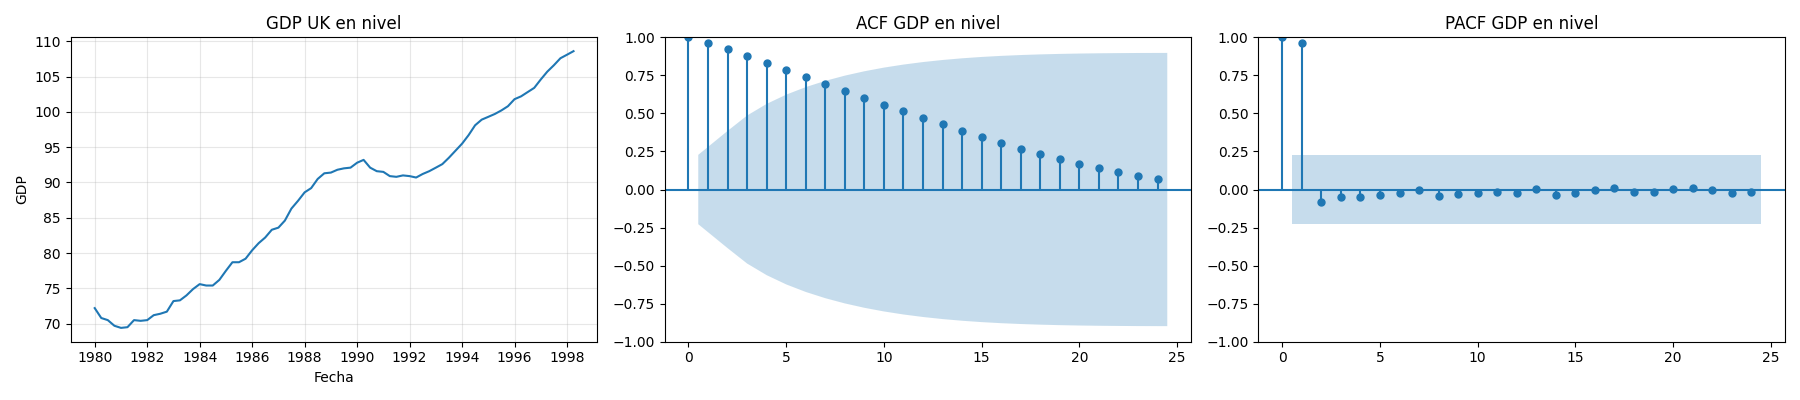
\includegraphics[width=0.9\textwidth]{grafico_1_GDP_ACF_PACF.png}		
	\caption{GDP ACF y PACF}
	\label{fig:diagnostico_residuos}		
	\end{figure}
	\begin{figure}[H]
	\centering		
	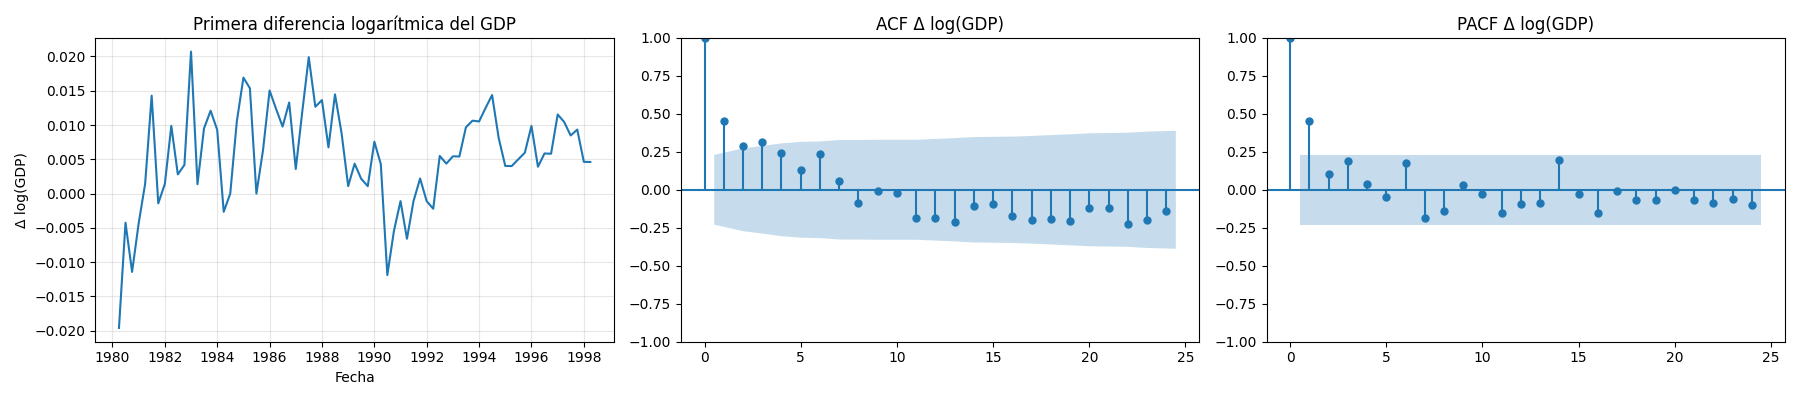
\includegraphics[width=0.9\textwidth]{grafico_2_Direfencia_Log_ACF_PACF.png}		
	\caption{Diferencia Logarítmica de ACF y PACF}
	\label{fig:diagnostico_residuos}		
	\end{figure}	
	
	
	Este resultado sugiere que la serie del GDP es integrada de orden uno, I(1), lo cual es consistente con la evidencia empírica en macroeconomía, donde las variables reales suelen exhibir alta persistencia. Desde el punto de vista metodológico, este diagnóstico es fundamental dentro del enfoque Box-Jenkins, ya que determina la necesidad de diferenciar la serie para lograr estacionariedad antes de proceder a la identificación y estimación de modelos ARIMA
	
	\subsection{Selección del modelo ARIMA}
	Dado que el análisis previo indica que la serie del GDP es integrada de orden uno, I(1), la modelación se realiza mediante especificaciones ARIMA(p,1,q), las cuales permiten capturar la dinámica de la serie una vez que esta ha sido diferenciada.
	
	De acuerdo con los resultados reportados en las Tablas:
	\begin{table}[H]
		\centering
		\caption{Comparación de Modelos ARIMA Candidatos}
		\label{tab:arima}
		
		\small
		
		\begin{tabular}{llrrrr}
			\toprule
			Modelo & Orden & AIC &	BIC & Log-Likelihood &	Durbin-Watson \\
			\midrule			
			ARIMA(1,1,1) &(1,1,1) &-527.4905 &-520.6191 &266.7453 &2.0677 \\			
			ARIMA(1,1,0) &(1,1,0) &-522.6666 &-518.0857 &263.3333 &	2.1871 \\			
			ARIMA(2,1,1) &(2,1,1) &-519.3491 &-510.1873 &263.6746 &	2.1896 \\			
			ARIMA(0,1,1) &(0,1,1) &-504.4093 &-499.8284 &254.2046 &	1.4687 \\			
			\bottomrule
		\end{tabular}
	\end{table}
	\begin{table}[H]
		\centering
		\caption{Significancia de Parámetros de Modelos ARIMA}
		\label{tab:significancia_arima}		
		\small		
		\begin{tabular}{llrrr}
			\toprule
			Modelo &Parámetro &Coeficiente &p-value &Sig. 5\% \\
			\midrule			
			ARIMA(1,1,0) &ar.L1 &0.6793 &0.0000 &True \\			
			ARIMA(1,1,0) &sigma2 &0.0000 &0.0000 &True \\			
			ARIMA(0,1,1) &ma.L1 &0.5172 &0.0000 &True \\			
			ARIMA(0,1,1) &sigma2 &0.0001 &0.0000 &True \\			
			ARIMA(1,1,1) &ar.L1 &0.8739 &0.0000 &True \\			
			ARIMA(1,1,1) &ma.L1 &-0.3565 &0.0183 &True \\			
			ARIMA(1,1,1) &sigma2 &0.0000 &0.0000 &True \\			
			ARIMA(2,1,1) &ar.L1 &0.2593 &0.8201 &False \\			
			ARIMA(2,1,1) &ar.L2 &0.3488 &0.6576 &False \\			
			ARIMA(2,1,1) &ma.L1 &0.3934 &0.7372 &False \\			
			\bottomrule
		\end{tabular}
	\end{table}
	Se evaluaron distintas combinaciones de componentes autorregresivos (AR) y de media móvil (MA). La selección del modelo se basa en criterios de información, particularmente el AIC y el BIC, así como en la significancia estadística de los parámetros estimados.
	
	En este contexto, el modelo ARIMA(1,1,1) presenta el mejor desempeño relativo, al ofrecer un balance adecuado entre ajuste y parsimonia, junto con parámetros estadísticamente significativos. Esto sugiere que la dinámica del GDP puede ser capturada mediante una combinación de efectos autorregresivos y de media móvil sobre la serie diferenciada.
	
	\subsection{Diagnóstico de Residuos}
	Con el objetivo de evaluar la adecuación del modelo seleccionado, se realiza un análisis de los residuos obtenidos a partir de la estimación del modelo ARIMA(1,1,1).
	
	En particular, se examina si los residuos se comportan como ruido blanco, condición necesaria para validar la correcta especificación del modelo.
	
	De acuerdo con los resultados reportados:
	\begin{table}[H]
		\centering
		\caption{Test Ljung-Box sobre Residuos del Modelo ARIMA}
		\label{tab:ljung_box}		
		\small		
		\begin{tabular}{rrr}
			\toprule
			Rezago &LB Statistic &p-value \\
			\midrule			
			4 &	0.0025 &1.0000 \\			
			8 &	0.0043 &1.0000 \\			
			12 &0.0057 &1.0000 \\			
			\bottomrule
		\end{tabular}
	
	\end{table}
	\begin{figure}[H]
		\centering		
		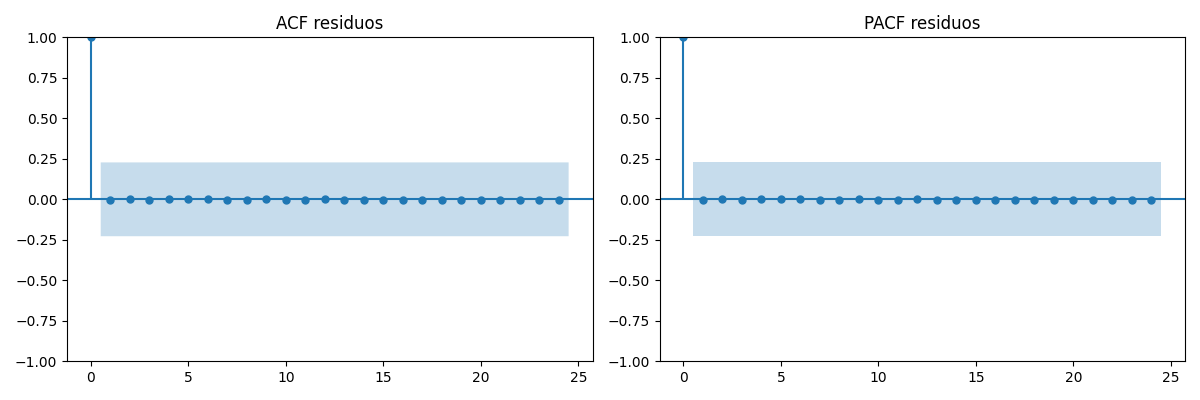
\includegraphics[width=0.9\textwidth]{grafico_4_Dicgnostico_de_Residuos.png}		
		\caption{Diagnóstico de residuos del modelo ARIMA seleccionado}
		\label{fig:diagnostico_residuos}		
	\end{figure}
	No se encuentra evidencia significativa de autocorrelación en los residuos. En efecto, el test de Ljung-Box no permite rechazar la hipótesis nula de ausencia de autocorrelación, lo que sugiere que la dependencia temporal ha sido adecuadamente capturada por el modelo.
	
	\subsection{Interpretación}
	La ausencia de autocorrelación residual indica que el modelo ARIMA(1,1,1) logra capturar de manera adecuada la estructura dinámica de la serie, cumpliendo con los supuestos fundamentales del enfoque Box-Jenkins. En otras palabras, no queda información sistemática en los residuos que pueda ser utilizada para mejorar la especificación del modelo.
	
	En este contexto, los residuos pueden considerarse aproximadamente como ruido blanco, lo que respalda la validez del modelo para fines de análisis y pronóstico.
	
	\subsection{Conclusión}
	Los resultados obtenidos indican que el modelo ARIMA(1,1,1) captura adecuadamente la dinámica del GDP, en la medida en que logra representar la persistencia de la serie una vez diferenciada y cumple con los supuestos fundamentales del enfoque Box-Jenkins.
	
	En particular, la selección del modelo se encuentra respaldada tanto por criterios de información como por la significancia estadística de sus parámetros, mientras que el análisis de residuos confirma la ausencia de autocorrelación remanente. Esto sugiere que el modelo logra capturar de manera satisfactoria la estructura temporal de la serie.
	
	En consecuencia, el modelo ARIMA(1,1,1) constituye una especificación adecuada para el análisis y pronóstico del GDP dentro del marco de series de tiempo, evidenciando la importancia de una correcta identificación, estimación y validación en la aplicación de la metodología Box-Jenkins.
	

	
	% =====================
	\section{Conclusión Final}
	
	El presente informe ha abordado el problema de la predictibilidad en series financieras desde una perspectiva integral, combinando simulaciones, evidencia empírica y modelación econométrica. 
	
	En la Parte 1, se mostró que la presencia de no estacionariedad puede generar inferencias inválidas a través de regresiones espurias, destacando la importancia de analizar las propiedades estadísticas de las series antes de estimar relaciones econométricas. En particular, se evidenció que la persistencia de los procesos incrementa la frecuencia de falsos rechazos, incluso en ausencia de relación económica entre las variables.
	
	En la Parte 2, se evaluó la hipótesis de commodity currencies, encontrando evidencia de predictibilidad en ejercicios in-sample consistente con la literatura. Sin embargo, los resultados out-of-sample mostraron un desempeño no robusto frente a benchmarks simples, y la evaluación económica indicó que dicha predictibilidad no se traduce en beneficios significativos en términos de estrategias de inversión. Estos resultados sugieren que la evidencia de predictibilidad es sensible a la especificación del modelo y al criterio de evaluación, lo que limita su aplicabilidad práctica.
	
	En la Parte 3, la aplicación de la metodología Box-Jenkins permitió modelar adecuadamente la dinámica del GDP, confirmando la presencia de integración de orden uno y la pertinencia de modelos ARIMA para capturar su comportamiento temporal. Asimismo, los diagnósticos de residuos respaldaron la validez de la especificación seleccionada, evidenciando la importancia de una correcta identificación y validación de modelos en series de tiempo.
	
	En conjunto, los resultados obtenidos refuerzan tres ideas fundamentales. Primero, la estacionariedad es un requisito esencial para la validez de la inferencia econométrica en series de tiempo. Segundo, la evaluación fuera de muestra constituye un criterio indispensable para validar la capacidad predictiva de los modelos. Tercero, la relevancia económica de la predictibilidad es un elemento clave que no siempre acompaña a la significancia estadística.
	
	En consecuencia, la evidencia sugiere que, si bien es posible identificar relaciones predictivas en contextos específicos, estas son generalmente frágiles, dependientes de la especificación y difíciles de explotar de manera sistemática en la práctica. Este resultado es consistente con la literatura en finanzas empíricas y subraya la importancia de un enfoque riguroso y crítico en el análisis predictivo.

	
\end{document}